\section{Additional post hoc comparisons}\label{sec:extended}
All comparisons in this section were designed after the original outcomes were available. They are descriptive, outside the original analysis rules, with unadjusted intervals; the pooled 59-contrast Holm audit is provided in the follow-up section. The original models, primary bootstrap rule, and evaluated cohorts are unchanged. Hyperparameter selection uses development families only. The corresponding plan, raw numerical inputs, predictions, per-episode iteration records, and executable scripts are included in release v0.4.0.

\subsection{Iterated nonlinear anchors}
The additional fit minimizes $\frac12\|u\|^2+64\sum_t\rho(\nu_t)$, where $u$ is the active physical displacement from the original prior in prior-scale units and $\nu_t$ is the nonlinear observation residual divided by its original observation standard deviation. Each IRLS step recomputes Huber weights $\min(1,1.345/|\nu_t|)$ or Cauchy weights $[1+(\nu_t/2.385)^2]^{-1}$, and solves the weighted nonlinear least-squares problem with the original Gaussian physical prior. This differs from the primary anchor's frozen weights based on the initial unit-update innovation. Sliding retains free initial position/velocity with bounds $[-5,5]$ m and $[0,10]$ m/s; general bounce retains height/velocity/floor bounds $[-0.5,2]$, $[-2,2]$, and $[-0.4,0.5]$ in SI units. Setup bounce uses its original known height/velocity and free offset. Gravity is fixed.

We initialize at the original anchor and prior, use the same observation-derived nuisance initialization, and select the lower objective without targets. Inner SciPy trust-region least squares uses function/step tolerances $10^{-12}$, gradient tolerance $10^{-10}$, and at most 150 function evaluations. The outer loop stops when physical prior-unit and nuisance-coordinate changes both have norm below $10^{-8}$, or at 50 iterations. The nonlinear bounce solution remains local. Both robust methods converge for all 1,440 distinct episode/bounce-setup assumption fits (slide results are reused across bounce-setup assumptions); mean outer counts are 3.117 for Huber and 4.508 for Cauchy. Median changes from the original anchor are $1.28\times10^{-6}$ and $1.72\times10^{-5}$ in prior units, although a small movement in strongly informed coordinates can affect the trajectory metric.

The profiled Gaussian comparison minimizes $\frac12\|u\|^2+\frac{n}{2}\log[\max(\sum_t\nu_t^2/n,10^{-12})]$ by L-BFGS-B using the same starts, bounds, and prior. The likelihood scale is profiled per episode and no scale prior is added. The floor is a numerical safeguard, not a fitted hyperparameter. No floor activation occurs; 1,438 of 1,440 fits report optimizer convergence. The two remaining fits are retained and flagged, so its result is a bounded numerical comparison, not an all-cases convergence claim. Its mean iteration count is 26.156. Original residual heads are never transferred to or retrained on these new anchors.
\begin{table}[htbp]\centering\small
\caption{Post hoc anchor comparisons; full minus baseline with 20,000 paired family draws. Units are millimeters.}\label{tab:ext_anchor}
\begin{tabular}{lrrrr}\toprule
Baseline & MAE & Reduction (\%) & Difference & 95\% interval\\\midrule
Iterated Huber & 1.914820 & 24.112 & -0.461698 & $[-0.663424,-0.269751]$\\
Iterated Cauchy & 1.913327 & 24.053 & -0.460205 & $[-0.661572,-0.268427]$\\
Profiled MAP & 1.823148 & 20.296 & -0.370027 & $[-0.562096,-0.183656]$\\
\bottomrule\end{tabular}
\end{table}
\subsection{Protocol and coordinate breakdown}
Each table entry first averages episodes within a family and protocol, then families equally. The arithmetic mean of all six action cells reproduces each method's saved macro error within $10^{-12}$ meters. Sliding rows are identical across bounce-setup assumptions, not independent replications. The protocol decomposition against the original cell-specific best-of-robust/legacy reference differs from comparison against Huber alone: sliding accounts for 99.9\% of that reduction and unforced sliding for 61.8\%.
\begin{table}[htbp]\centering\small
\caption{Complete action decomposition (mm). G/S denote general/setup bounce-setup assumptions; M/U/B denote multiple-force, unforced, and bounce protocols.}\label{tab:ext_protocol}
\begin{tabular}{lrrrrrr}\toprule
Method & G-M & G-U & G-B & S-M & S-U & S-B\\\midrule
Unit & 3.633112 & 2.156062 & 0.791835 & 3.633112 & 2.156062 & 0.344740\\
Fixed Huber & 3.633112 & 2.156062 & 0.515000 & 3.633112 & 2.156062 & 0.352266\\
Fixed Cauchy & 3.638990 & 2.169002 & 0.516761 & 3.638990 & 2.169002 & 0.355631\\
Numerical & 3.020342 & 0.977727 & 0.515000 & 3.020342 & 0.977727 & 0.301482\\
Full & 2.989925 & 0.960083 & 0.515000 & 2.989925 & 0.960083 & 0.303715\\
Legacy & 3.901642 & 2.002216 & 0.792138 & 3.901642 & 2.002216 & 0.307627\\
RGB temporal & 4.249430 & 2.344330 & 0.782657 & 4.249430 & 2.344330 & 0.335869\\
Iterated Huber & 3.068313 & 2.086893 & 0.833767 & 3.068313 & 2.086893 & 0.344740\\
Iterated Cauchy & 3.068283 & 2.086901 & 0.824849 & 3.068283 & 2.086901 & 0.344743\\
Profiled MAP & 2.893515 & 2.071250 & 0.664873 & 2.893515 & 2.071250 & 0.344488\\
\bottomrule\end{tabular}
\end{table}
Coordinate errors below show family-macro mean / median of family mean absolute transformed-coordinate error. Inactive coordinates are N/A. Shared sliding rows are shown once; the downloadable CSV also contains their duplicate setup-bounce-setup assumption rows. This table measures estimation error, not nuisance error or an identifiability guarantee.
\begingroup\scriptsize
\begin{longtable}{llrrr}
\caption{Active-coordinate error by method and protocol.}\\
\toprule Method & Protocol & $\log m$ & $\log\mu$ & $\operatorname{logit}e$\\\midrule\endhead
Unit & Multiple & 0.04640 / 0.03933 & 0.05513 / 0.04507 & N/A\\
Unit & Unforced & N/A & 0.01371 / 0.01033 & N/A\\
Unit & General B & N/A & N/A & 0.01257 / 0.00359\\
Unit & Setup B & N/A & N/A & 0.00394 / 0.00300\\
Fixed Huber & Multiple & 0.04640 / 0.03933 & 0.05513 / 0.04507 & N/A\\
Fixed Huber & Unforced & N/A & 0.01371 / 0.01033 & N/A\\
Fixed Huber & General B & N/A & N/A & 0.00506 / 0.00301\\
Fixed Huber & Setup B & N/A & N/A & 0.00414 / 0.00302\\
Fixed Cauchy & Multiple & 0.04652 / 0.03953 & 0.05525 / 0.04565 & N/A\\
Fixed Cauchy & Unforced & N/A & 0.01380 / 0.01033 & N/A\\
Fixed Cauchy & General B & N/A & N/A & 0.00506 / 0.00307\\
Fixed Cauchy & Setup B & N/A & N/A & 0.00420 / 0.00307\\
Numerical & Multiple & 0.03147 / 0.02499 & 0.03182 / 0.02460 & N/A\\
Numerical & Unforced & N/A & 0.00633 / 0.00584 & N/A\\
Numerical & General B & N/A & N/A & 0.00506 / 0.00301\\
Numerical & Setup B & N/A & N/A & 0.00328 / 0.00267\\
Full & Multiple & 0.03111 / 0.02488 & 0.03177 / 0.02355 & N/A\\
Full & Unforced & N/A & 0.00619 / 0.00544 & N/A\\
Full & General B & N/A & N/A & 0.00506 / 0.00301\\
Full & Setup B & N/A & N/A & 0.00330 / 0.00266\\
Legacy & Multiple & 0.05082 / 0.04345 & 0.05874 / 0.05118 & N/A\\
Legacy & Unforced & N/A & 0.01239 / 0.01032 & N/A\\
Legacy & General B & N/A & N/A & 0.01266 / 0.00386\\
Legacy & Setup B & N/A & N/A & 0.00321 / 0.00276\\
RGB temporal & Multiple & 0.05361 / 0.04449 & 0.06527 / 0.05126 & N/A\\
RGB temporal & Unforced & N/A & 0.01461 / 0.01035 & N/A\\
RGB temporal & General B & N/A & N/A & 0.01248 / 0.00362\\
RGB temporal & Setup B & N/A & N/A & 0.00377 / 0.00312\\
Iterated Huber & Multiple & 0.03998 / 0.03512 & 0.04470 / 0.03547 & N/A\\
Iterated Huber & Unforced & N/A & 0.01321 / 0.00991 & N/A\\
Iterated Huber & General B & N/A & N/A & 0.01352 / 0.00361\\
Iterated Huber & Setup B & N/A & N/A & 0.00394 / 0.00300\\
Iterated Cauchy & Multiple & 0.03999 / 0.03514 & 0.04470 / 0.03548 & N/A\\
Iterated Cauchy & Unforced & N/A & 0.01321 / 0.00990 & N/A\\
Iterated Cauchy & General B & N/A & N/A & 0.01353 / 0.00353\\
Iterated Cauchy & Setup B & N/A & N/A & 0.00394 / 0.00300\\
Profiled MAP & Multiple & 0.03819 / 0.03086 & 0.04294 / 0.03579 & N/A\\
Profiled MAP & Unforced & N/A & 0.01309 / 0.01038 & N/A\\
Profiled MAP & General B & N/A & N/A & 0.00697 / 0.00321\\
Profiled MAP & Setup B & N/A & N/A & 0.00394 / 0.00300\\
\bottomrule\end{longtable}\endgroup
\subsection{Cross-fitted targets and shrinkage}
Five family-disjoint inner folds create numerical predictions for the visual targets inside each of six outer development folds. The final descriptive model uses five inner folds across all development families, then fits numerical and visual coefficients on all development data. Inner numerical normalization uses only its training families. Visual normalization uses the outer training data, as in the original model. Ridge penalties, masks, clipping, and shrinkage are fixed. The only changed learning target is the residual after an out-of-fold numerical prediction. No evaluated-family targets enter fitting or selection.
\begin{table}[htbp]\centering\small
\caption{Visual increment under the two target constructions. Intervals are paired differences from numerical-only, in mm.}\label{tab:ext_crossfit}
\begin{tabular}{lrrrr}\toprule
Cohort & Target & MAE & Increment (\%) & 95\% interval\\\midrule
Development & in sample & 1.352231 & 1.436 & $[-0.03773,-0.00131]$\\
Confirmation & in sample & 1.453122 & 1.065 & $[-0.03114,+0.00053]$\\
Development & crossfit & 1.350328 & 1.574 & $[-0.04228,-0.00046]$\\
Confirmation & crossfit & 1.451620 & 1.168 & $[-0.03446,+0.00095]$\\
\bottomrule\end{tabular}
\end{table}
The corresponding one-sided upper bounds on evaluated families are $-0.002189$ mm (original targets) and $-0.002213$ mm (cross-fitted targets). Both two-sided intervals include zero. The original full view improves 46/72 families; the exact two-sided binomial sign test is $p=0.02446$. That frequency null differs from the mean-difference bootstrap null, so the sign result is not substituted for the mean inference.

The shrinkage sweep changes only the fixed multiplier of the already clipped visual prediction; its training target and fitted coefficients are unchanged. Covariance is recomputed from the accepted total correction. The original 0.25 row reproduces the original full predictions and all scores to $10^{-12}$. The development point minimum at 0.50 does not trigger replacement of the original model.
\begin{table}[htbp]\centering\small
\caption{Post hoc visual-shrinkage sensitivity. Development is six-fold; evaluated results are descriptive.}\label{tab:ext_shrink}
\begin{tabular}{lrrrrr}\toprule
Cohort & Scale & MAE (mm) & NLL/dim. & CRPS & Coverage\\\midrule
Development & 0 & 1.371928 & -2.175173 & 0.013604 & 0.975000\\
Development & 0.1 & 1.362306 & -2.177212 & 0.013603 & 0.975000\\
Development & 0.25 & 1.352231 & -2.179550 & 0.013619 & 0.975505\\
Development & 0.5 & 1.347138 & -2.181497 & 0.013691 & 0.975000\\
Development & 1.0 & 1.385694 & -2.177991 & 0.014000 & 0.973485\\
Confirmation & 0 & 1.468770 & -2.542391 & 0.013136 & 0.973611\\
Confirmation & 0.1 & 1.460132 & -2.544056 & 0.013122 & 0.973611\\
Confirmation & 0.25 & 1.453122 & -2.545938 & 0.013113 & 0.973611\\
Confirmation & 0.5 & 1.447645 & -2.547442 & 0.013133 & 0.973611\\
Confirmation & 1.0 & 1.465189 & -2.544428 & 0.013299 & 0.974537\\
\bottomrule\end{tabular}
\end{table}
\subsection{Development-selected channels and direct regressors}
Combined, pooled-only, and position-only views each search penalties $\{1,10,100\}$ using six-fold development macro action error. The selected penalties are 10, 1, and 1. Dimension-specific columns are removed rather than padded; training means and standard deviations are recomputed within folds. Selection reuses development outcomes, so selected development scores are not unbiased generalization estimates. All evaluated-cohort comparisons remain descriptive. The full nine-point search is in \path{replayed/extended/channel_grid.csv}.

The deduplicated numerical view uses the nine varying channels at eight frames plus the 15 setup channels once, totaling 87. It searches $\{0.1,1,10\}$, selects 0.1, and retains the visual stage. This sensitivity does not replace the original 192-dimensional view. The original replication of constants effectively distributes regularization over repeated columns.
\begin{table}[htbp]\centering\small
\caption{Development-selected feature views; evaluated differences and intervals are relative to numerical-only. Units are mm.}\label{tab:ext_channels}
\begin{tabular}{lrrrr}\toprule
View & Penalty & Develop. & Evaluated & 95\% interval\\\midrule
full & 10 & 1.352231 & 1.453122 & $[-0.03114,+0.00053]$\\
pooled & 1 & 1.367114 & 1.467461 & $[-0.01873,+0.01721]$\\
position & 1 & 1.351154 & 1.451117 & $[-0.03101,-0.00512]$\\
deduplicated numeric & 0.1 & 1.347917 & 1.426315 & $[-0.07105,-0.01508]$\\
\bottomrule\end{tabular}
\end{table}
Direct ridge and MLP use the same 240 numerical-plus-visual input coordinates and predict all three transformed properties, without an anchor update or output mask. Known setup/prior information remains in the input features. Ridge penalties $\{0.1,1,10,100,1000\}$ are selected by five inner family folds inside each outer training set. The direct MLP has two 64-unit ReLU hidden layers and three outputs, AdamW with learning rate 0.001 and weight decay $10^{-4}$, and a 300-epoch cap. Training-family normalization is used for inputs and raw-coordinate targets; no anchor-standardized target is used. One of five inner family folds selects the epoch by standardized-coordinate MSE with patience 25, then all outer training families are refitted at that epoch. Seeds 17, 43, and 101 are averaged in prediction space. Final selected epochs are 60, 84, and 80. These are specified small-network baselines, not an exhaustive learned-system comparison, and no posterior is supplied.
\begin{table}[htbp]\centering\small
\caption{Post hoc direct-regression baselines. Difference intervals are relative to the original full model, in mm.}\label{tab:ext_direct}
\begin{tabular}{lrrr}\toprule
Method & Cohort & MAE & 95\% difference interval\\\midrule
RIDGE & Development & 32.399926 & $[28.51888,33.64795]$\\
RIDGE & Confirmation & 33.402860 & $[28.75547,35.34003]$\\
MLP & Development & 30.620605 & $[26.38529,32.34098]$\\
MLP & Confirmation & 26.489233 & $[22.42777,27.73870]$\\
\bottomrule\end{tabular}
\end{table}
\subsection{Engine-rollout proxy}
PyBullet DIRECT simulates a 0.01-m-radius sphere with zero rotational inertia, a plane with unit friction and restitution, zero damping, and estimated/true object coefficients. Gravity is 9.81 m/s$^2$, time step $1/480$ s, solver iterations 100, and restitution velocity threshold zero. The same force schedule, initial speeds, drop height, and eight evaluation times as the analytic metric are used. No image rendering or new observation extraction is needed: this is a downstream simulation of saved estimates. It is a nonrotating-contact proxy rather than a rerendering or dynamic validation of the original geometry assets. The plane/object coefficients combine through the engine's contact model. The saved engine trajectories and family losses allow independent metric replay without PyBullet; fresh rollouts require PyBullet (tested Linux build January 29, 2025, API 202010061).
\begin{table}[htbp]\centering\small
\caption{Controlled engine proxy and analytic metric, aggregated by family.}\label{tab:ext_engine}
\begin{tabular}{lrrrr}\toprule
Method & Engine MAE (mm) & Analytic MAE (mm) & Pearson & Spearman\\\midrule
Fixed Huber & 2.236155 & 2.074269 & 0.99251 & 0.98566\\
Numerical & 1.620483 & 1.468770 & 0.98035 & 0.96128\\
Full & 1.605715 & 1.453122 & 0.97954 & 0.96373\\
\bottomrule\end{tabular}
\end{table}
The full-minus-Huber paired interval is $[-0.83816,-0.44089]$ mm. Agreement of family rankings supports the analytic proxy within this controlled contact model, not independent real-world accuracy.
\begin{figure}[htbp]\centering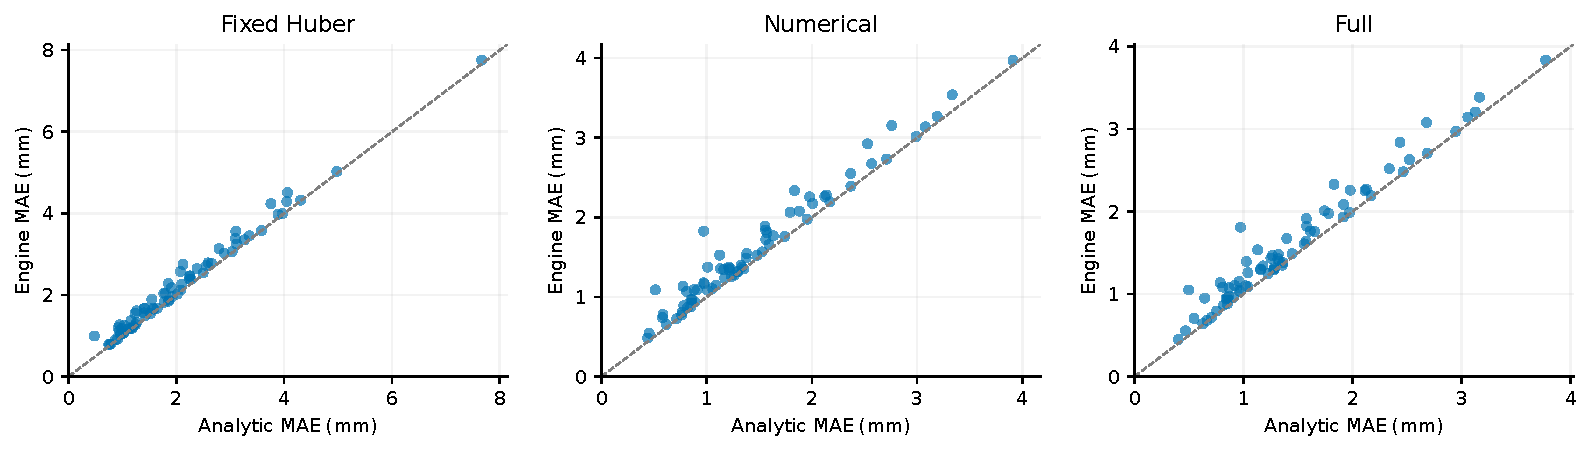
\includegraphics[width=.95\textwidth]{figures/engine_scatter.pdf}\caption{Post hoc family-level analytic and controlled-engine errors. Each panel has 72 families; no family is removed.}\end{figure}

\subsection{Public displacement scales}
Normalized MAE divides episode mean vector error by mean target-vector norm. Vector $R^2=1-\sum_i\|\hat y_i-y_i\|^2/\sum_i\|y_i-\bar y\|^2$. These are episode-weighted descriptors, separate from the primary equal-material-pair MAE. A mean predictor fitted on development may have slightly negative evaluation $R^2$; a predictor set to the evaluation mean is an oracle sanity check with exactly zero $R^2$, not a baseline selected on evaluation targets.
\begin{table}[htbp]\centering\small
\caption{Target displacement-norm distribution (mm).}\label{tab:ext_scale}
\begin{tabular}{lrrrrrr}\toprule
Split & n & Mean & Median & SD & Q25 & Q75\\\midrule
Episode & 123 & 193.869 & 215.989 & 64.589 & 179.374 & 229.273\\
Material & 329 & 190.281 & 213.097 & 57.974 & 170.110 & 226.632\\
\bottomrule\end{tabular}
\end{table}
\begin{table}[htbp]\centering\small
\caption{Episode-normalized public errors and vector coefficients of determination.}\label{tab:ext_r2}
\begin{tabular}{lrrr}\toprule
Split & Method & Normalized MAE & $R^2$\\\midrule
Episode & constant prior & 0.681551 & -0.004428\\
Episode & numeric & 0.382638 & 0.621118\\
Episode & raw vlm & 0.367309 & 0.661853\\
Episode & gated vlm & 0.366303 & 0.658853\\
Material & numeric & 0.342079 & 0.634251\\
Material & raw & 0.339718 & 0.649059\\
Material & gated & 0.329793 & 0.657154\\
\bottomrule\end{tabular}
\end{table}
\subsection{Recorded inference-time components}
One hundred outcome-free selected episodes (34 multiple-force, 33 unforced, 33 bounce) are measured at batch size one, with CUDA synchronization around GPU stages. Model loading is excluded; totals sum components measured in separate model-resident passes. They are not contiguous cold-start or deployment throughput benchmarks. The shared first-image prior remains in both paths; a fully VLM-free baseline would be a different model. Tracking/initialization includes its required image work, and visual preprocessing includes its own image loading. Hardware: NVIDIA GeForce RTX 5080, driver 591.86, CUDA 12.8, PyTorch 2.11.0+cu128, Python 3.11.9, Windows build 26200. The setup-bounce row uses only its 33 applicable episodes and is already included in the robust-fit total, not added twice.
\begin{table}[htbp]\centering\small
\caption{Measured latency components (milliseconds); 100 episodes except the setup-bounce subset.}\label{tab:ext_latency}
\begin{tabular}{lrrr}\toprule
Stage & Median & Q25 & Q75\\\midrule
First-image prior & 68.394 & 60.705 & 81.938\\
Additional frame preprocessing & 15.747 & 15.373 & 16.096\\
Eight-frame vision encoder & 179.167 & 177.558 & 181.665\\
Observation decoder & 32.741 & 31.952 & 40.214\\
Tracking / initialization & 37.570 & 36.221 & 51.689\\
Robust fits, both bounce-setup assumptions & 17.523 & 16.159 & 43.753\\
Setup bounce, 75 calls (subset) & 16.869 & 16.643 & 17.350\\
Residual heads & 0.342 & 0.319 & 0.353\\
Shared-prior / anchor component sum & 129.067 & 117.546 & 163.849\\
Full component sum & 362.528 & 345.832 & 396.436\\
\bottomrule\end{tabular}
\end{table}
The exact measurement source and all 100 timing rows are retained. Portable replay verifies those recorded quantiles; it does not recreate timings on a different computer. New measurement requires the source's original RGB inputs and upstream model environment. General bounce uses 81 forward evaluations in the original kernel, whereas setup bounce uses 75; these distinct budgets are not conflated.

\subsection{Bounce and real-video diagnostics}
The bounce diagnostics compare the unclamped branch's learned standardized correction with its true standardized target, without changing the deployed fallback. Fold-wise correlations, clipping rates, scales, and target dispersion are provided in \path{replayed/extended/bounce_diagnostics.csv}. The evaluated rows are shown below. Training numerical clipping rate is zero for the full development fit; visual prediction clipping occurs only in general bounce. Similar median anchor scales alongside very different residual-target dispersion favor a predictability explanation over an unsupported claim of uniformly inflated covariance. The role of free nuisance coordinates is not causally isolated.
\begin{table}[htbp]\centering\small
\caption{Evaluated bounce residual diagnostics; each bounce-setup assumption has 360 episodes.}\label{tab:ext_bounce}
\begin{tabular}{lrrrr}\toprule
Bounce setup & Correlation & Visual clip rate & Median scale & Target SD\\\midrule
Generalized & 0.185769 & 0.063889 & 0.007517 & 2.264421\\
Setup & 0.501755 & 0.000000 & 0.007098 & 0.571314\\
\bottomrule\end{tabular}
\end{table}
The original real-video diagnostic is a scalar feature score, not a physical-property prediction, and does not invoke the appearance prior. Its mean (0.05614) and SD (0.04048) differ from the synthetic unforced visual score (0.00619 and 0.02482), but their motion-feature units are not matched: real inputs use projected pixels and synthetic inputs use shifts divided by tracking noise. This contract difference is directly visible in the supplied extraction sources. Therefore a calibrated property-distribution comparison and attribution of failure to the appearance prior are not applicable to this diagnostic.

The combined, pooled-only, and position-only real-score family correlations are $-0.700$, 0.027, and $-0.455$. The recorded 95\% family-bootstrap interval for the combined score is $[-0.972,-0.108]$. Tracking uses MIL with an overlay-derived initial cue, not red-component segmentation. The recorded tracker failure count is zero on 33 videos; its effectively fixed-size boxes cannot validate object-size accuracy. Saved centroid second-difference roughness has Spearman 0.558 with family absolute rank error, but this is an unlabeled smoothness proxy, not a ground-truth tracking-error measurement or a causal explanation. The follow-up section corrects the noise-normalization contract and reruns these scores; the negative combined ranking persists. Independent tracking labels and a new evaluation cohort are still required for causal attribution.
